%\documentclass[mathserif]{beamer}
\documentclass[handout]{beamer}
%\usetheme{Goettingen}
\usetheme{Warsaw}
%\usetheme{Singapore}
%\usetheme{Frankfurt}
%\usetheme{Copenhagen}
%\usetheme{Szeged}
%\usetheme{Montpellier}
%\usetheme{CambridgeUS}
%\usecolortheme{}
%\setbeamercovered{transparent}
\usepackage[english, activeacute]{babel}
\usepackage[utf8]{inputenc}
\usepackage{amsmath, amssymb}
\usepackage{dsfont}
\usepackage{graphics}
\usepackage{cases}
\usepackage{graphicx}
\usepackage{pgf}
\usepackage{epsfig}
\usepackage{amssymb}
\usepackage{multirow}	
\usepackage{amstext}
\usepackage[ruled,vlined,lined]{algorithm2e}
\usepackage{amsmath}
\usepackage{epic}
\usepackage{epsfig}
\usepackage{fontenc}
\usepackage{framed,color}
\usepackage{palatino, url, multicol}
\usepackage{listings}
%\algsetup{indent=2em}


\vspace{-0.5cm}
\title{Summarizing the Posterior}
\vspace{-0.5cm}
\author[Felipe Bravo Márquez]{\footnotesize
%\author{\footnotesize  
 \textcolor[rgb]{0.00,0.00,1.00}{Felipe José Bravo Márquez}} 
\date{ \today }




\begin{document}
\begin{frame}
\titlepage


\end{frame}


%%%%%%%%%%%%%%%%%%%%%%%%%%%


\begin{frame}{Summarizing the Posterior}
\scriptsize{
\begin{itemize}

\item Once our Bayesian model produces a posterior distribution, it is necessary to summarize and interpret it.

\item However, a posterior distribution is (usually) a high dimensional object that is hard to visualize and work with \cite{pml1Book}.

\item In this class we will learn how to draw estimates (e.g., point estimates, intervals, predictions) to summarize and interpret a posterior distribution.



\item Exactly how it is summarized depends upon our purpose.

\item Common questions include:
\begin{itemize}
\begin{scriptsize}
 \item How much posterior probability lies below some parameter value?
 \item How much posterior probability lies between two parameter values?
 \item Which parameter value marks the lower 5\% of the posterior probability?
 \item Which range of parameter values contains 90\% of the posterior probability?
 \item Which parameter value has highest posterior probability?
 \end{scriptsize}
\end{itemize}
 
\end{itemize}



} 

\end{frame}


\begin{frame}{Sampling to summarize}
\scriptsize{
\begin{itemize}

\item These questions can be usefully divided into questions about: 
\begin{itemize}
\scriptsize{
 \item intervals of defined boundaries
 \item intervals of defined probability area
 \item point estimates
}
\end{itemize}
 
\item In the theoretical world (when the posterior has a closed mathematical expressions), answering these questions implies calculating complicated integrals to cancel out (or average) different variables.

\item In the practical world, however, the same results can be approximated  using \textbf{samples} from the posterior. 
 
\item In this class we will approach the above questions using samples from the posterior. 

\item Another reason to learn to work with posterior samples is that methods like MCMC produce nothing but samples from the posterior.


\item This class is based on Chapter 3 of \cite{mcelreath2020statistical}.

\end{itemize}
}

\end{frame}










\begin{frame}[fragile]{Sampling from a grid-approximate posterior}
\scriptsize{
\begin{itemize}

\item Before beginning to work with samples, we need to generate them.

\item Here’s a reminder for how to compute the posterior for the globe tossing model, using grid approximation:

\begin{verbatim}
p_grid <- seq( from=0 , to=1 , length.out=1000 )
prior <- rep( 1 , 1000 )
likelihood <- dbinom( 6 , size=9 , prob=p_grid )
posterior <- likelihood * prior
posterior <- posterior / sum(posterior)
\end{verbatim}

\item Now we wish to draw 10,000 samples from this posterior. 

\item Imagine the posterior is a bucket full of parameter values, numbers such as 0.1, 0.7, 0.5, 1, etc.

\item Within the bucket, each value exists in proportion to its posterior probability, such that values near the peak are much more common than those in the tails. 
 
\end{itemize}



} 

\end{frame}



\begin{frame}[fragile]{Sampling from a grid-approximate posterior}
\scriptsize{
\begin{itemize}

\item We’re going to scoop out 10,000 values from the bucket.

\item Provided the bucket is well mixed, the resulting samples will have the same proportions as the exact posterior density. 

\item Therefore the individual values of $p$ will appear in our samples in proportion to the posterior plausibility of each value.

\item Here’s how you can do this in R, with one line of code:

\begin{verbatim}
samples <- sample( p_grid , prob=posterior , size=1e4 , 
replace=TRUE )
\end{verbatim}
\item We are randomly pulling values from the grid of parameter values where the probability of each value is given by the posterior.

 
\end{itemize}



} 

\end{frame}


\begin{frame}[fragile]{Sampling from a grid-approximate posterior}
\scriptsize{
\begin{itemize}

\item We can visualize a density plot of our posterior sample as follows:

\begin{verbatim}
library(rethinking)
dens(samples) 
\end{verbatim}

   \begin{figure}[h!]
	\centering
	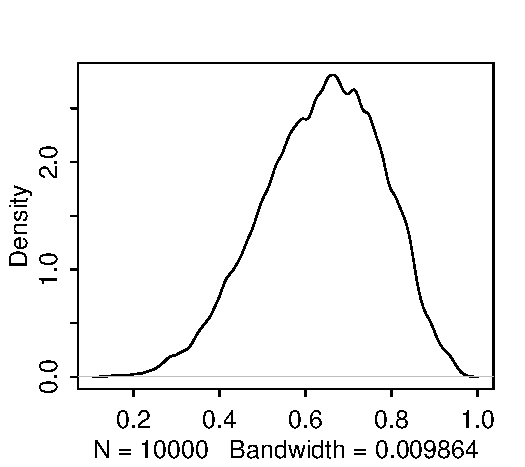
\includegraphics[scale=0.7]{pics/posteriorTossGrid.pdf}
	\end{figure} 
 




\item We can see that the estimated density is very similar to to ideal posterior we computed via grid approximation in previous class.


 
\end{itemize}



} 

\end{frame}


\begin{frame}[fragile]{Sampling from the theoretical posterior}
\scriptsize{
\begin{itemize}

\item We could get very similar results by sampling from the theoretical posterior using the beta distribution: 

\begin{verbatim}
teo.samples<-rbeta(1e4,7,4)
dens(teo.samples)
\end{verbatim}



   \begin{figure}[h!]
	\centering
	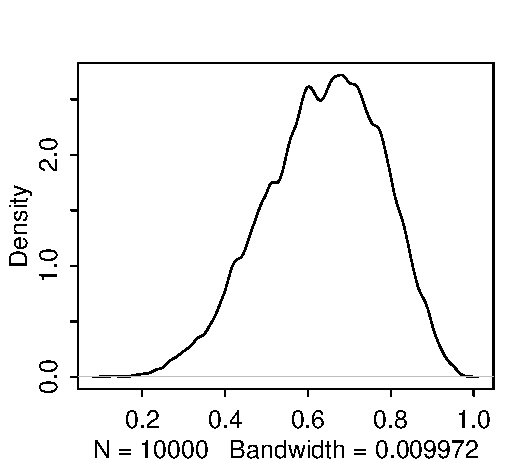
\includegraphics[scale=0.6]{pics/posteriorTossBeta.pdf}
	\end{figure} 

	
\item We can see that the samples of the grid-approximated posterior and the theoretical posterior are indistinguishable.
	

\item However, we should keep in mind that for complex models we will not have access to the posterior closed form.
\end{itemize}



} 

\end{frame}

\begin{frame}[fragile]{Intervals of defined boundaries}
\scriptsize{
\begin{itemize}

\item Suppose we are asked for the posterior probability that the proportion of water is less than 0.5. 

\item We could calculate this from the theoretical posterior:

\begin{verbatim}
> pbeta(0.5,7,4)
[1] 0.171875
\end{verbatim}



\item Or alternatively we could calculate it from the grid-approximate posterior by adding up all of the probabilities where the corresponding parameter value is less than 0.5.

\begin{verbatim}
> sum( posterior[ p_grid < 0.5 ] )
[1] 0.1718746
\end{verbatim}


\item So about 17\% of the posterior probability is below 0.5.

\end{itemize}



} 

\end{frame}



\begin{frame}{Intervals of defined boundaries}
\scriptsize{

   \begin{figure}[h!]
	\centering
	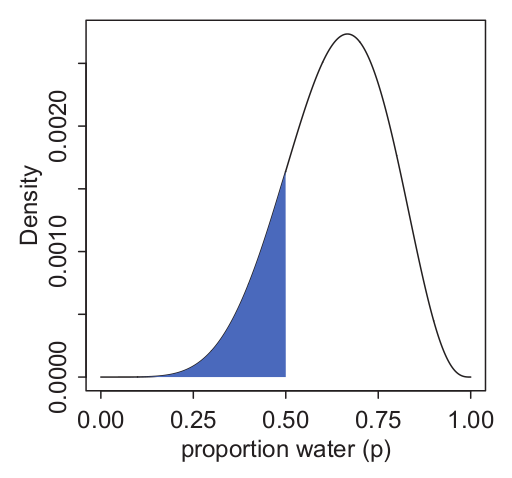
\includegraphics[scale=0.45]{pics/interval1.png}
	\end{figure} 




} 

\end{frame}


\begin{frame}[fragile]{Intervals of defined boundaries}
\scriptsize{
\begin{itemize}

\item Now, let's perform the same calculation, using samples from the posterior.

\item Recall than in more complex models neither a grid-approximation nor a closed-form posterior will be available.

\item All we have to do is add up all samples less than 0.5 and divide the resulting count by the total number of samples.

\begin{verbatim}
> sum( samples < 0.5 ) / 1e4
[1] 0.1752 
\end{verbatim}


\item In R, the condition \verb+samples < 0.5+ returns a logical vector, so since R treats TRUE values as 1, \verb+sum+ will count all the samples satisfying the condition.

\end{itemize}



} 

\end{frame}


\begin{frame}[fragile]{Intervals of defined boundaries}
\scriptsize{
\begin{itemize}

\item Now, we can ask our sample how much posterior probability lies between 0.5 and 0.75.

\begin{verbatim}
> sum( samples > 0.5 & samples < 0.75 ) / 1e4
[1] 0.6043
\end{verbatim}

\item So about 61\% of the posterior probability lies between 0.5 and 0.75.

\item Let's validate this result using the exact posterior:

\begin{verbatim}
> pbeta(0.75,7,4)-pbeta(0.5,7,4)
[1] 0.6040001
\end{verbatim}

\end{itemize}



} 

\end{frame}

\begin{frame}{Intervals of defined boundaries}
\scriptsize{

   \begin{figure}[h!]
	\centering
	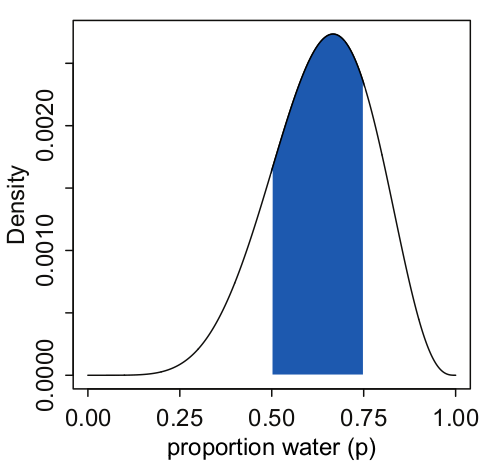
\includegraphics[scale=0.45]{pics/interval2.png}
	\end{figure} 




} 

\end{frame}




\begin{frame}[fragile]{Intervals of defined probability}
\scriptsize{
\begin{itemize}

\item Suppose we want to know the boundaries of the lower 80\% posterior probability.

\item We can answer this by obtaining the 80-th percentile of the posterior sample:

\begin{verbatim}
> quantile( samples , 0.8 )
      80% 
0.7577578 
\end{verbatim}

\item Or alternatively, using the quantile function of the beta distribution (the distribution of the exact posterior):


\begin{verbatim}
> qbeta(0.8,7,4 )
[1] 0.7605588 
\end{verbatim}

\end{itemize}


} 

\end{frame}



\begin{frame}{Intervals of defined probability}
\scriptsize{

   \begin{figure}[h!]
	\centering
	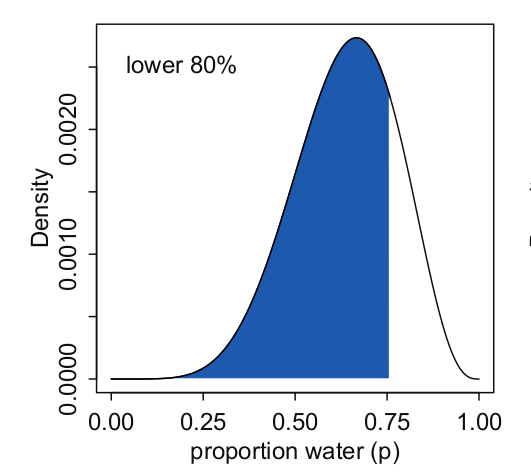
\includegraphics[scale=0.45]{pics/interval3.png}
	\end{figure} 




} 

\end{frame}



\begin{frame}[fragile]{Intervals of defined probability}
\scriptsize{
\begin{itemize}

\item Similarly, we can calculate the middle 80\% interval that lies between the 10th percentile and the 90th percentile: 


\begin{verbatim}
> quantile( samples , c( 0.1 , 0.9 ) )
      10%       90% 
0.4504505 0.8148148 
\end{verbatim}



\item The ``rethinking'' package provides the function \verb+PI+ (from percentile interval) to calculate this type of interval:

\begin{verbatim}
> PI( samples , prob=0.8 )
      10%       90% 
0.4504505 0.8148148 
\end{verbatim}

\item Notice that we are assigning $(1-0.8)/2=0.1$ of probability above and below the interval.

\item We can also obtain the exact interval from the exact posterior:


\begin{verbatim}
> c("10%"=qbeta(0.1,7,4 ),"90%"=qbeta(0.9,7,4 ))
      10%       90% 
0.4482692 0.8124377 
\end{verbatim}

\end{itemize}


} 

\end{frame}



\begin{frame}{Intervals of defined probability}
\scriptsize{

   \begin{figure}[h!]
	\centering
	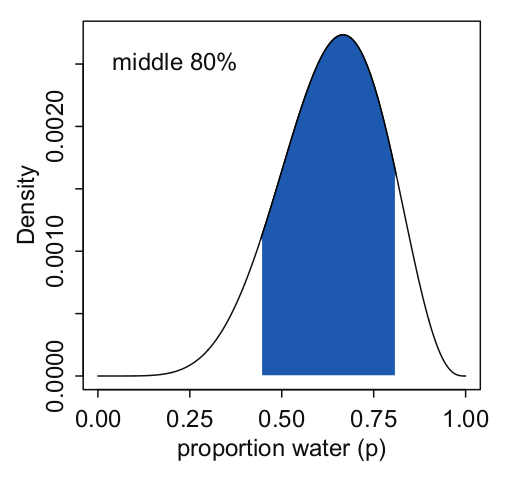
\includegraphics[scale=0.45]{pics/interval4.png}
	\end{figure} 




} 

\end{frame}


\begin{frame}[fragile]{Credible Intervals}
\scriptsize{
\begin{itemize}

\item The intervals of posterior probability that assign equal probability to each tail are called \textbf{credible intervals}.

\item These posterior intervals report two parameter values that contain between them a specified amount of posterior probability.

\item What the interval indicates is a range of parameter values compatible with the model and data.

\item Credible intervals resemble very much the confidence intervals seen in previous lectures on frequentist inference.

\item The interpretations are very different though.

\item A confidence interval is a region\footnote{Notice that the region will vary from one experiment to another.} that after infinitely repeating the data sampling experiment will contain the true parameter with a certain frequency.


\item In contrast, a credible interval is a range of values that we believe our parameter can take with a certain probability according to both our prior beliefs and the evidence given by the data.

\end{itemize}



} 

\end{frame}


\begin{frame}[fragile]{Credible Intervals}
\scriptsize{
\begin{itemize}

\item Equal-tailed credible intervals do a good job of communicating the shape of a distribution, as long as the distribution isn't too asymmetrical.

\item Suppose that in our globe tossing experiment we had observed 3 W and 0 L.

\item If we again consider a flat prior, we will get a highly skewed posterior distribution with its maximum value at the boundary, $p = 1$.

\begin{verbatim}
  p_grid.a <- seq( from=0 , to=1 , length.out=1000 )
  prior.a <- rep(1,1000)
  likelihood.a <- dbinom( 3 , size=3 , prob=p_grid.a )
  posterior.a <- likelihood.a * prior.a
  posterior.a <- posterior.a / sum(posterior.a)
  samples.a <- sample( p_grid.a , size=1e4 , 
  replace=TRUE , prob=posterior.a )
  dens(samples.a,xlim=c(0,0.935))
\end{verbatim}

\item Alternatively we could sample from the exact posterior $Beta(\alpha + W , \beta + L)$ = $Beta(1 + 3 , 1 + 0)$ = $Beta(4,1)$:

\begin{verbatim}
  teo.samples.a<-rbeta(1e4,4,1)
  dens(teo.samples.a,xlim=c(0,0.935))
\end{verbatim}


\end{itemize}



} 

\end{frame}

\begin{frame}{Credible Intervals}
\scriptsize{

   \begin{figure}[h!]
	\centering
	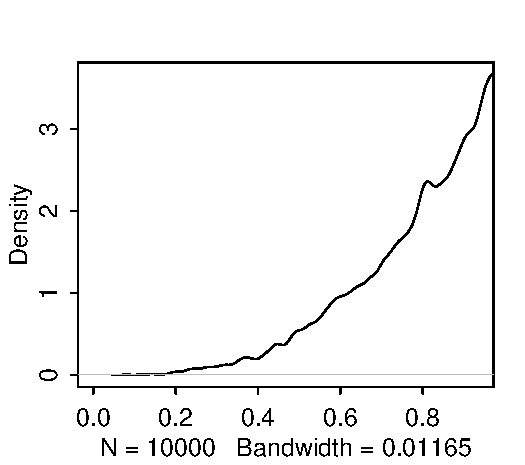
\includegraphics[scale=0.91]{pics/post_asy.pdf}
	\end{figure} 




} 

\end{frame}

\begin{frame}[fragile]{Credible Intervals}
\scriptsize{
\begin{itemize}

\item Let's compute a 50\%  equal-tailed credible interval for this posterior:

\begin{verbatim}
> PI( samples.a , prob=0.5 )  
      25%       75% 
0.7037037 0.9309309 
\end{verbatim}

\item This interval assigns 25\% of the probability area above and below the interval. 

\item So it provides the central 50\% probability. 

\item But in this example, it ends up excluding the most probable parameter values, near $p = 1$.

\item So, in terms of describing the shape of the posterior distribution it can be misleading.


\end{itemize}



} 

\end{frame}


\begin{frame}{Credible Intervals}
\scriptsize{

   \begin{figure}[h!]
	\centering
	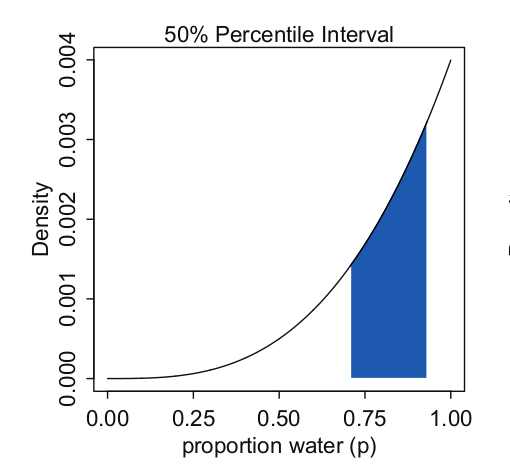
\includegraphics[scale=0.45]{pics/interval5.png}
	\end{figure} 




} 

\end{frame}


\begin{frame}[fragile]{Highest Posterior Density Intervals}
\scriptsize{
\begin{itemize}

\item An alternative type of credible interval is the Highest Posterior Density Interval (HPDI).

\item If we relax the restriction of assigning equal probability to each tail, we obtain an infinite number of intervals containing the specified probability area.

\item The HPDI is the narrowest of those possible interval.

\item It can be calculated from posterior samples using the HPDI function from the rethinking package.

\begin{verbatim}
> HPDI( samples.a , prob=0.5 )
     |0.5      0.5| 
0.8368368 1.0000000  
\end{verbatim}

\item This interval captures the parameters with highest posterior probability, as well as being noticeably narrower: 0.16 in width rather than 0.23 for the equal-tailed credible interval.

\end{itemize}



} 

\end{frame}


\begin{frame}{Highest Posterior Density Intervals}
\scriptsize{

   \begin{figure}[h!]
	\centering
	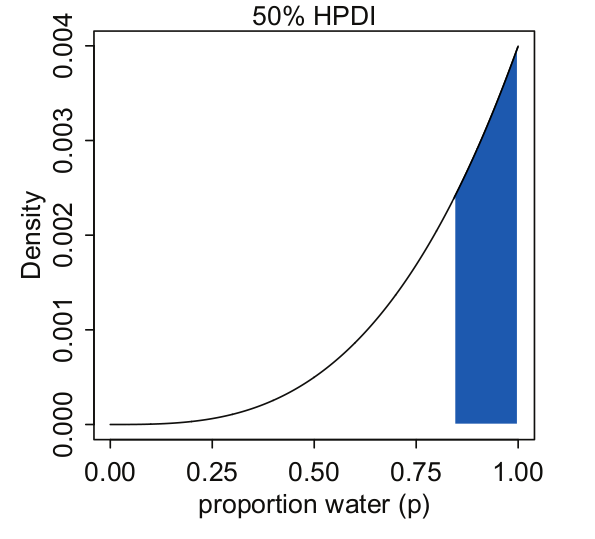
\includegraphics[scale=0.4]{pics/interval6.png}
	\end{figure} 




} 
\end{frame}


\begin{frame}[fragile]{Highest Posterior Density Intervals}
\scriptsize{
\begin{itemize}

\item A disadvantage of the HPDI, is that it is more computationally intensive than the equal-tailed credible interval.

\item Apart from the cases when the posterior distribution is highly skewed, these two types of intervals are similar.

\item For example, let's calculate an 80\% HPDI for the the original posterior with 6 W and 3 L:

\begin{verbatim}
> HPDI( samples , prob=0.8 )
     |0.8      0.8| 
0.4694695 0.8298298  
\end{verbatim}

\item This interval is very similar to the equal-tailed credible interval calculated before.


\end{itemize}



} 

\end{frame}



\begin{frame}{Point estimates}
\scriptsize{
\begin{itemize}

\item The idea of point estimation in a Bayesian setting is to summarize the posterior with a single value. 

\item The three most common options here:

\begin{itemize}
\scriptsize{
 \item The mode, which is the value with highest posterior probability, also known as the maximum a posteriori (MAP) estimate.
 \item The mean
 \item The median
} 
\end{itemize}

\item Let's calculate them for the globe tossing experiment in which we observe 3 waters out of 3 tosses.



\end{itemize}



} 

\end{frame}



\begin{frame}[fragile]{Point estimates}
\scriptsize{
\begin{itemize}

\item We can compute the MAP from the grid approximation of the posterior as follows:

\begin{verbatim}
 > p_grid[ which.max(posterior.a) ]
[1] 1
\end{verbatim}


\item Or we can approximate it using posterior samples:

\begin{verbatim}
> dd <- density(samples.a,adj=0.01)
> dd$x[which.max(dd$y)]
[1] 0.9971593 
\end{verbatim}

\item The same procedure can be done more easily using the chainmode function from the rethinking package:

\begin{verbatim}
> chainmode( samples.a , adj=0.01 )
[1] 0.9971593 
\end{verbatim}





\end{itemize}



} 

\end{frame}



\begin{frame}[fragile]{Point estimates}
\scriptsize{
\begin{itemize}

\item Now the posterior mean:

\begin{verbatim}
> mean(samples.a)
[1] 0.7988011
\end{verbatim}


\item and the median:

\begin{verbatim}
> median(samples.a)
[1] 0.8408408
\end{verbatim}


\item Which of these values should we report?

\item Recall that our ultimate goal is to report the shape of the posterior.

\item Hence, it is better to communicate as much as we can about it.  

\item This can include: density plots, HPDI, MAP estimates, mean, mode, etc..


\end{itemize}



} 

\end{frame}

\begin{frame}{Point Estimates}
\scriptsize{

   \begin{figure}[h!]
	\centering
	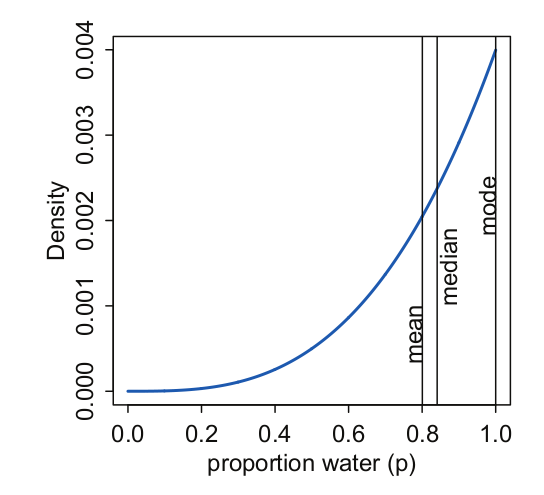
\includegraphics[scale=0.45]{pics/posterior_points.png}
	\end{figure} 




} 

\end{frame}


\begin{frame}{Sampling to Simulate Prediction}
\scriptsize{

\begin{itemize}
\item Another useful thing we can do with the posterior, is to use it to simulate new data predictions.

\item This can be particularly useful for evaluating our model in an empirical way.

\item The idea is to contrast the simulated data with the expected behavior.

\item These simulated predictions can also be used to forecast future observations.

\item But, we must recall that the posterior is a distribution of the parameter given the data $f(\theta|d)$, so how can we use it to generate new unseen observations $\tilde{d}$?

\item To understand this, we need to learn about the \textbf{posterior predictive distribution}.

\item But before introducing this complex new concept, we will learn how to generate simulated predictions using  the likelihood function of the model.

\end{itemize}


} 
\end{frame}


\begin{frame}[fragile]{Sampling to Simulate Prediction}
\scriptsize{

\begin{itemize}
\item In our original globe tossing experiment, the MAP estimate (the value of $p$ that maximizes the posterior) was $0.67$.

\item We can use the likelihood function (a Binomial in this case) with $p=0.67$ to generate new observations of waters  $\tilde{d}$ with 9 new tosses.

\begin{verbatim}
> rbinom( 1, size=9 , prob=0.67)
[1] 6 
\end{verbatim}

\item In this new data, we obtained 6 W out of 9 tosses, which is an expected behavior considering that the original data also had 6 W (out of 9).

\item Now, we can repeat this process 100,000 times and observe a sampling distribution for the number of waters obtained:

\begin{verbatim}
> new_w <- rbinom( 1e5 , size=9 , prob=0.67 )
> simplehist( new_w , xlab="new water predictions") 
\end{verbatim}




\end{itemize}


} 
\end{frame}





\begin{frame}{Sampling to Simulate Prediction}
\scriptsize{

   \begin{figure}[h!]
	\centering
	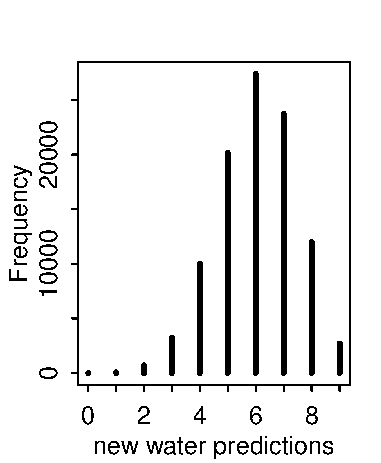
\includegraphics{pics/w_predictions.pdf}
	\end{figure} 




} 

\end{frame}


\begin{frame}{Sampling to Simulate Prediction}
\scriptsize{

\begin{itemize}

\item We can see that even 6 W is the most frequent case, 7 and 5 are also very likely to occur in our sampling distribution.

\item These predictions embody the observation uncertainty: for a given value of $p$ the number of W may vary according to our likelihood function (unless $p=0$ or $p=1$) .

\item But there is an additional source of uncertainty that our current predictions are not taking into account: the uncertainty about $p$.

\item The posterior distribution over $p$ embodies this uncertainty.

\item And since there is uncertainty about $p$, there is uncertainty about everything that depends upon $p$.

\item We loss this information when we pluck out a single parameter value (e.g., the MAP estimate) and then perform calculations with it. 


\end{itemize}


} 
\end{frame}



\begin{frame}{Posterior Predictive Distribution}
\scriptsize{

\begin{itemize}

\item This loss of information leads to overconfidence.

\item  We'd like to propagate the parameter uncertainty as we evaluate the
implied predictions.

\item All that is required is averaging over the posterior density for $p$, while computing the predictions.

\item For each possible value of the parameter $p$, there is an implied
distribution of outcomes.

\item So if you were to compute the sampling distribution of outcomes at each value of $p$, then you could average all of these prediction distributions together, using the posterior probabilities of each value of $p$, to get a \textbf{posterior predictive distribution}.
\end{itemize}


} 
\end{frame}


\begin{frame}{Posterior Predictive Distribution}

   \begin{figure}[h!]
	\centering
	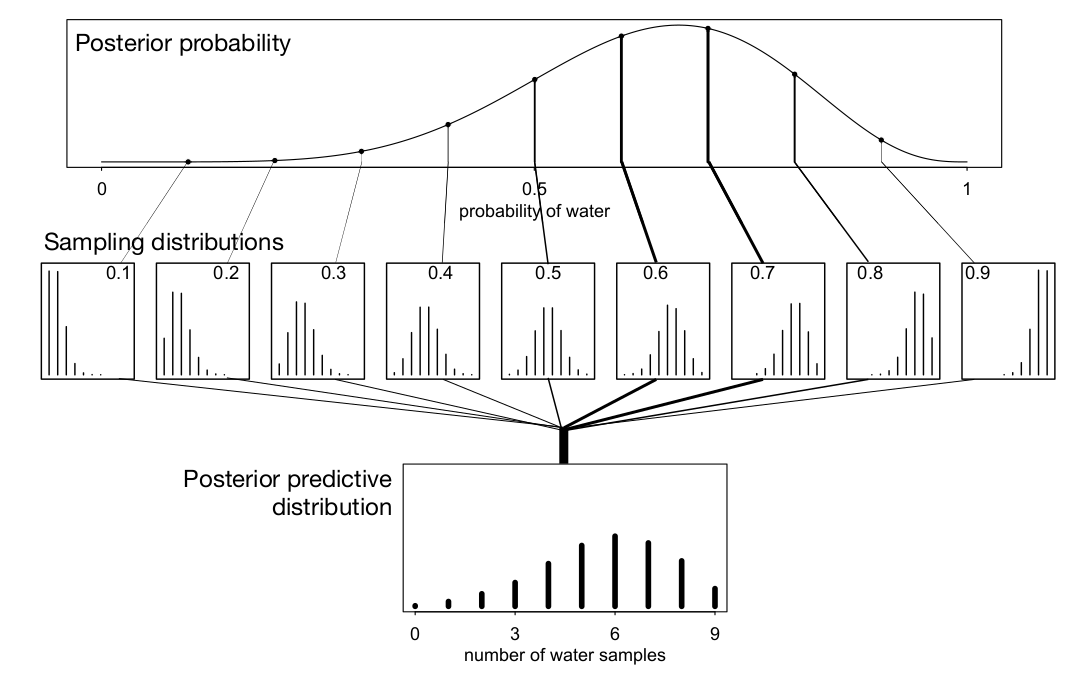
\includegraphics[scale=0.31]{pics/posterior_predictive.png}
	\end{figure} 

\end{frame}


\begin{frame}{Posterior Predictive Distribution}
\scriptsize{

\begin{itemize}

\item  The figure above illustrates this averaging. 

\item At the top, the posterior distribution is shown, with 10 unique parameter values highlighted by the vertical lines. 

\item The implied distribution of observations specific to each of these parameter values is shown in the middle row of plots. 

\item Observations are never certain for any value of $p$, but they do shift around in response to it. 

\item Finally, at the bottom, the sampling distributions for all values of p are combined, using the posterior probabilities to compute the weighted average frequency of each possible observation, zero to nine water samples.

\item The resulting distribution is for predictions, but it incorporates all of the uncertainty embodied in the posterior distribution for the parameter $p$. 

\item As a result, it is more honest than the distribution of predictions computed with the MAP estimate.



\end{itemize}


} 
\end{frame}


\begin{frame}[fragile]{Posterior Predictive Distribution}
\scriptsize{

\begin{itemize}

\item Generating predictions with the MAP estimate can lead us to believe that the model is more consistent with the data than it really is.

\item This illusion arises from tossing away uncertainty about the parameters. 

\item Consequently, MAP predictions tend to cluster around the observations more tightly (i.e., produce narrower distributions). 

\item  To generate predictions using the Posterior Predictive Distribution in R, we must replace the MAP parameter value with samples from the posterior:

\begin{verbatim}
> post_pred_w <- rbinom( 1e4 , size=9 , prob=samples )
> simplehist( post_pred_w , xlab="posterior predictions")
\end{verbatim}


\item For each sampled value, a random binomial observation is generated.

\item Since the sampled values appear in proportion to their posterior probabilities, the resulting simulated observations are averaged over the posterior.


\end{itemize}


} 
\end{frame}


\begin{frame}{Posterior Predictive Distribution}

   \begin{figure}[h!]
	\centering
	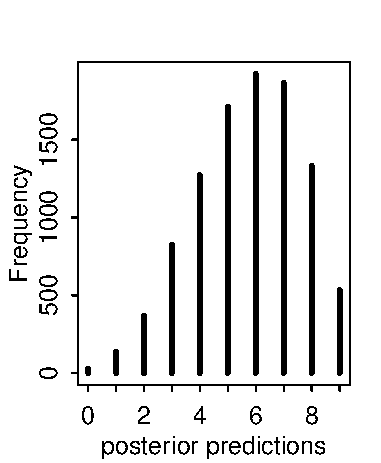
\includegraphics{pics/w_post_predictions.pdf}
	\end{figure} 

\end{frame}


\begin{frame}{Posterior Predictive Distribution}
\scriptsize{

\begin{itemize}

\item Let's discuss the posterior predictive distribution more formally as presented in \cite{gelman2013bayesian}.

 \item After the data $d$ have been observed, we can predict an unknown observable $\tilde{d}$ from the same process.
 
 \item In the globe tossing experiment $\tilde{d}$ may be the yet to be recorded number of waters W in a new tossing experiment.
 
 \item The distribution of  $\tilde{d}$ given $d$ is called the \textbf{posterior predictive distribution}.
 
 \item Posterior because it is conditional on the observed $d$ and predictive because it is a prediction for an observable $\tilde{d}$. 
 
 
 
\end{itemize}



} 
\end{frame}





\begin{frame}{Posterior Predictive Distribution}
\scriptsize{


\begin{itemize}
 
\item Mathematical, the posterior predictive distribution is defined as follows:

  \begin{eqnarray*}
 f(\tilde{d}|d) & = & \int_{\theta}f(\tilde{d},\theta|d)d\theta \\ 
                & = &  \int_{\theta}f(\tilde{d}|\theta,d)f(\theta|d)d\theta \\
                & = &  \int_{\theta}f(\tilde{d}|\theta)f(\theta|d)d\theta \\
 \end{eqnarray*}
 
 \item The second and third lines display the posterior predictive distribution as an average of conditional predictions over the posterior distribution of $\theta$.
 
 \item The last step follows from the assumed conditional independence of $d$ and $\tilde{d}$ given $\theta$.
 
 
 
\end{itemize}










} 
\end{frame}







\begin{frame}{Conclusions}
\scriptsize{

\begin{itemize}
\item In this class we introduced the basic procedures for manipulating posterior distributions.
\item Our fundamental tool is samples of parameter values drawn from the posterior distribution.
\item Working with samples transforms a problem of integral calculus into a problem of data summary. 
\item These samples can be used to produce intervals, point estimates, posterior predictive checks, as well as other kinds of simulations.
\item Posterior predictive checks combine uncertainty about parameters, as described by the posterior distribution, with uncertainty about outcomes, as described by the assumed likelihood function. 
\item These checks are useful for analyzing the behavior of the model.
\end{itemize}


} 
\end{frame}


%%%%%%%%%%%%%%%%%%%%%%%%%%%
\begin{frame}[allowframebreaks]\scriptsize
\frametitle{References}
\bibliography{bio}
\bibliographystyle{apalike}
%\bibliographystyle{flexbib}
\end{frame}  









%%%%%%%%%%%%%%%%%%%%%%%%%%%

\end{document}
